\chapter{Experimental Results and Analysis}

This chapter reports the outcomes of the two experimental stages and analyzes the findings against the hypotheses established in Chapter~3. The presentation follows the experimental structure: first the broad screening results from Stage~1, then the focused deep-dive results from Stage~2, and finally a synthesis of findings across both stages.

\section{Stage 1: Broad Screening Results}

Stage~1 evaluated four feature selection strategies across four datasets and three model families, producing 7,920 individual observations in the summarized outputs. This section presents aggregate findings organized by research question.

\subsection{Predictive Performance}

Table~\ref{tab:stage1_best} reports the best-performing strategy for each dataset-model combination, determined by minimum mean RMSE across all retention levels.

\begin{table}[h]
\centering
\caption{Best RMSE by dataset and model in Stage~1, showing winning strategy and retention level.}
\label{tab:stage1_best}
\begin{tabular}{llllr}
\toprule
\textbf{Dataset} & \textbf{Model} & \textbf{Best Strategy} & \textbf{k} & \textbf{RMSE} \\
\midrule
Allstate Claims & Ridge & MI & 1.00 & 2090.07 \\
Allstate Claims & ExtraTrees & MI & 1.00 & 1992.76 \\
Allstate Claims & XGBoost & SHAP & 0.50 & 1897.11 \\
\midrule
Bike Sharing & Ridge & MI & 1.00 & 141.04 \\
Bike Sharing & ExtraTrees & MI & 1.00 & 40.83 \\
Bike Sharing & XGBoost & MI & 1.00 & 42.57 \\
\midrule
Communities \& Crime & Ridge & MI & 1.00 & 0.136 \\
Communities \& Crime & ExtraTrees & Tree-FI & 0.50 & 0.134 \\
Communities \& Crime & XGBoost & SHAP & 0.75 & 0.138 \\
\midrule
Superconductor & Ridge & MI & 1.00 & 17.65 \\
Superconductor & ExtraTrees & MI & 0.75 & 9.11 \\
Superconductor & XGBoost & Tree-FI & 0.75 & 9.98 \\
\bottomrule
\end{tabular}
\end{table}

Several patterns emerge from this summary:

\textbf{No universal winner}: As hypothesized (H1), no single strategy dominates all configurations. The winning method varies by dataset and model, confirming that feature selection effectiveness is context-dependent.

\textbf{MI frequently competitive}: Mutual Information achieves the best result in 7 of 12 configurations, often at $k=1.00$ (full feature set). This suggests that for some dataset-model pairs, feature selection provides no benefit over using all features, and MI's ranking at least does not harm performance.

\textbf{SHAP wins selectively}: SHAP achieves the best RMSE in 2 configurations, both with XGBoost---Allstate at $k=0.50$ and Communities and Crime at $k=0.75$. These wins occur at intermediate retention levels, consistent with hypothesis H2.

\textbf{Tree-FI competitive for tree models}: Tree-based importance wins in 2 configurations, both with tree-based models (ExtraTrees on Communities, XGBoost on Superconductor).

Figure~\ref{fig:stage1_rmse} visualizes RMSE by strategy across datasets, illustrating the variability in method rankings.

\begin{figure}[h]
    \centering
    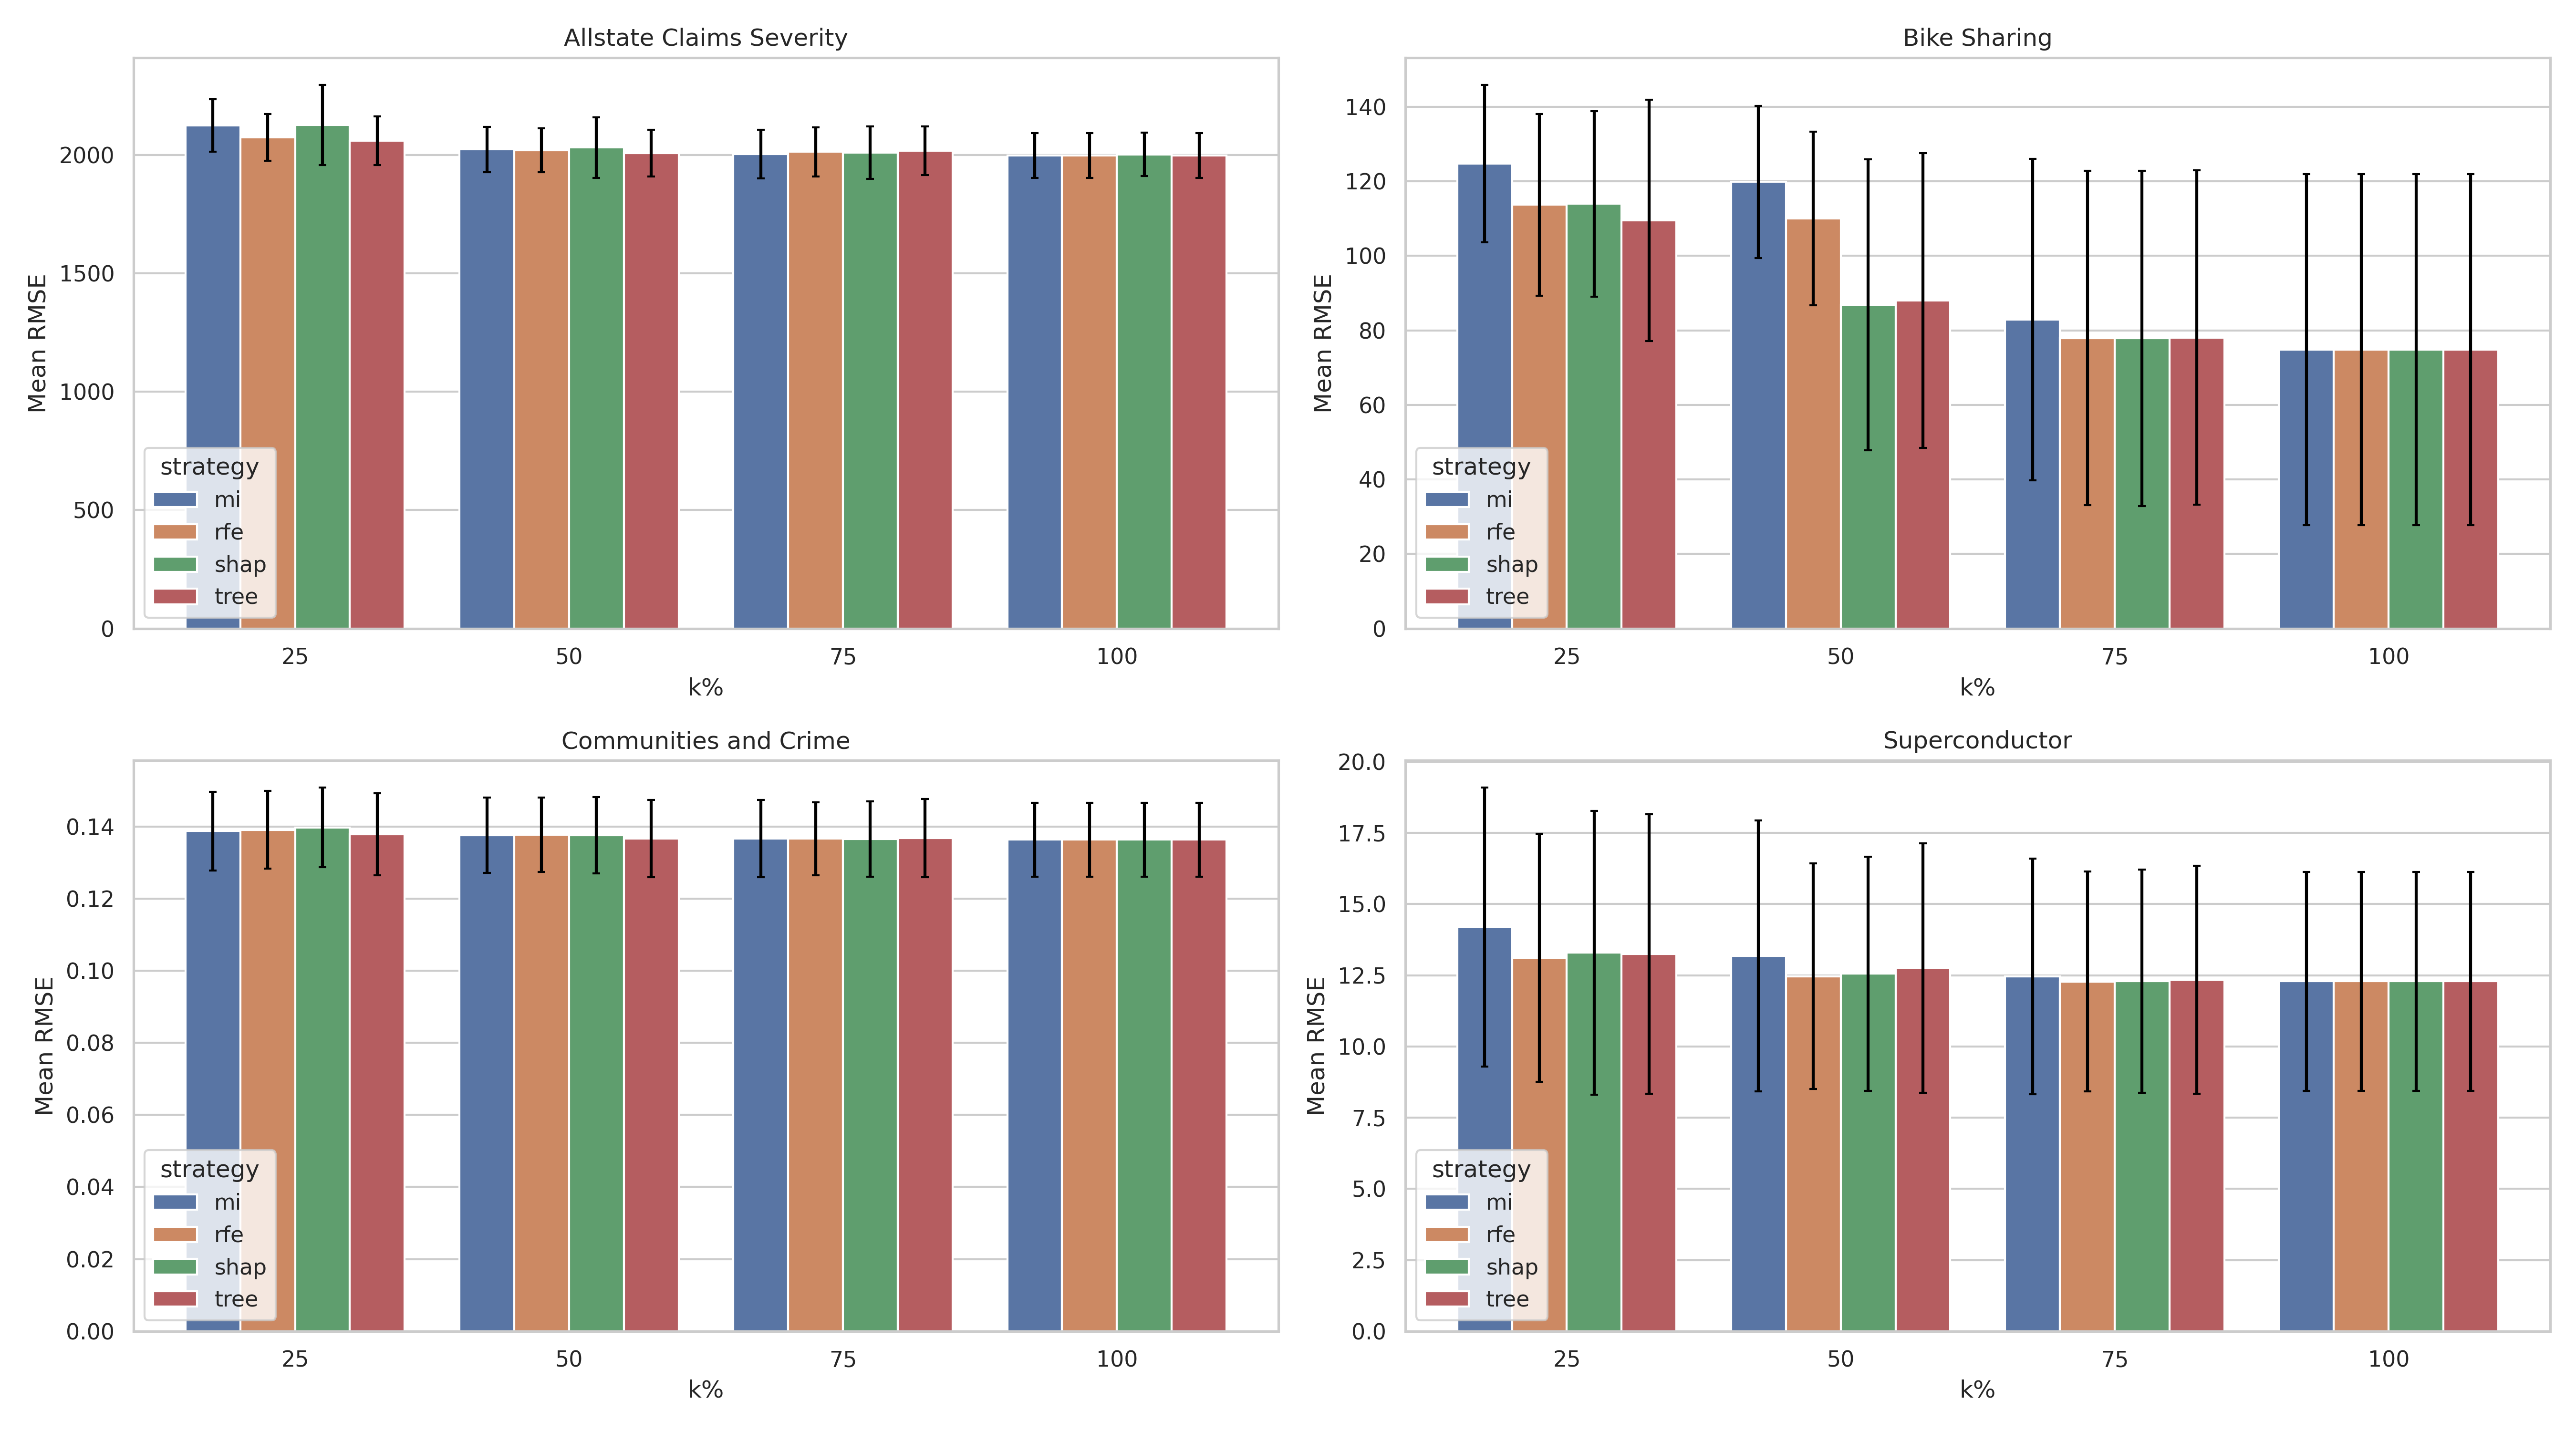
\includegraphics[width=0.85\textwidth]{../runs/exp1_plus_big-arff-run/figures/fig1_rmse_by_strategy_all_2x2.png}
    \caption{Stage~1 RMSE comparison by strategy across all four datasets.}
    \label{fig:stage1_rmse}
\end{figure}

\subsection{Computational Cost}

Table~\ref{tab:stage1_cost} presents average selection time by strategy and model family, aggregated across datasets and retention levels.

\begin{table}[h]
\centering
\caption{Mean selection time (seconds) by strategy and model in Stage~1.}
\label{tab:stage1_cost}
\begin{tabular}{lrrr}
\toprule
\textbf{Strategy} & \textbf{Ridge} & \textbf{ExtraTrees} & \textbf{XGBoost} \\
\midrule
MI & 0.75 & 0.82 & 0.72 \\
RFE & 0.27 & 0.16 & 0.26 \\
Tree-FI & 0.60 & 0.77 & 0.53 \\
SHAP & 0.01 & 5.42 & 0.54 \\
\bottomrule
\end{tabular}
\end{table}

The cost patterns reveal nuance: SHAP selection time varies dramatically by model. For Ridge, SHAP computation is near-instantaneous (linear SHAP is fast). For ExtraTrees, SHAP incurs substantial overhead---roughly 6-7x the cost of MI. For XGBoost, the TreeExplainer efficiency keeps SHAP competitive with other methods.

Figure~\ref{fig:stage1_cost} shows the full distribution of computational costs across configurations.

\begin{figure}[h]
    \centering
    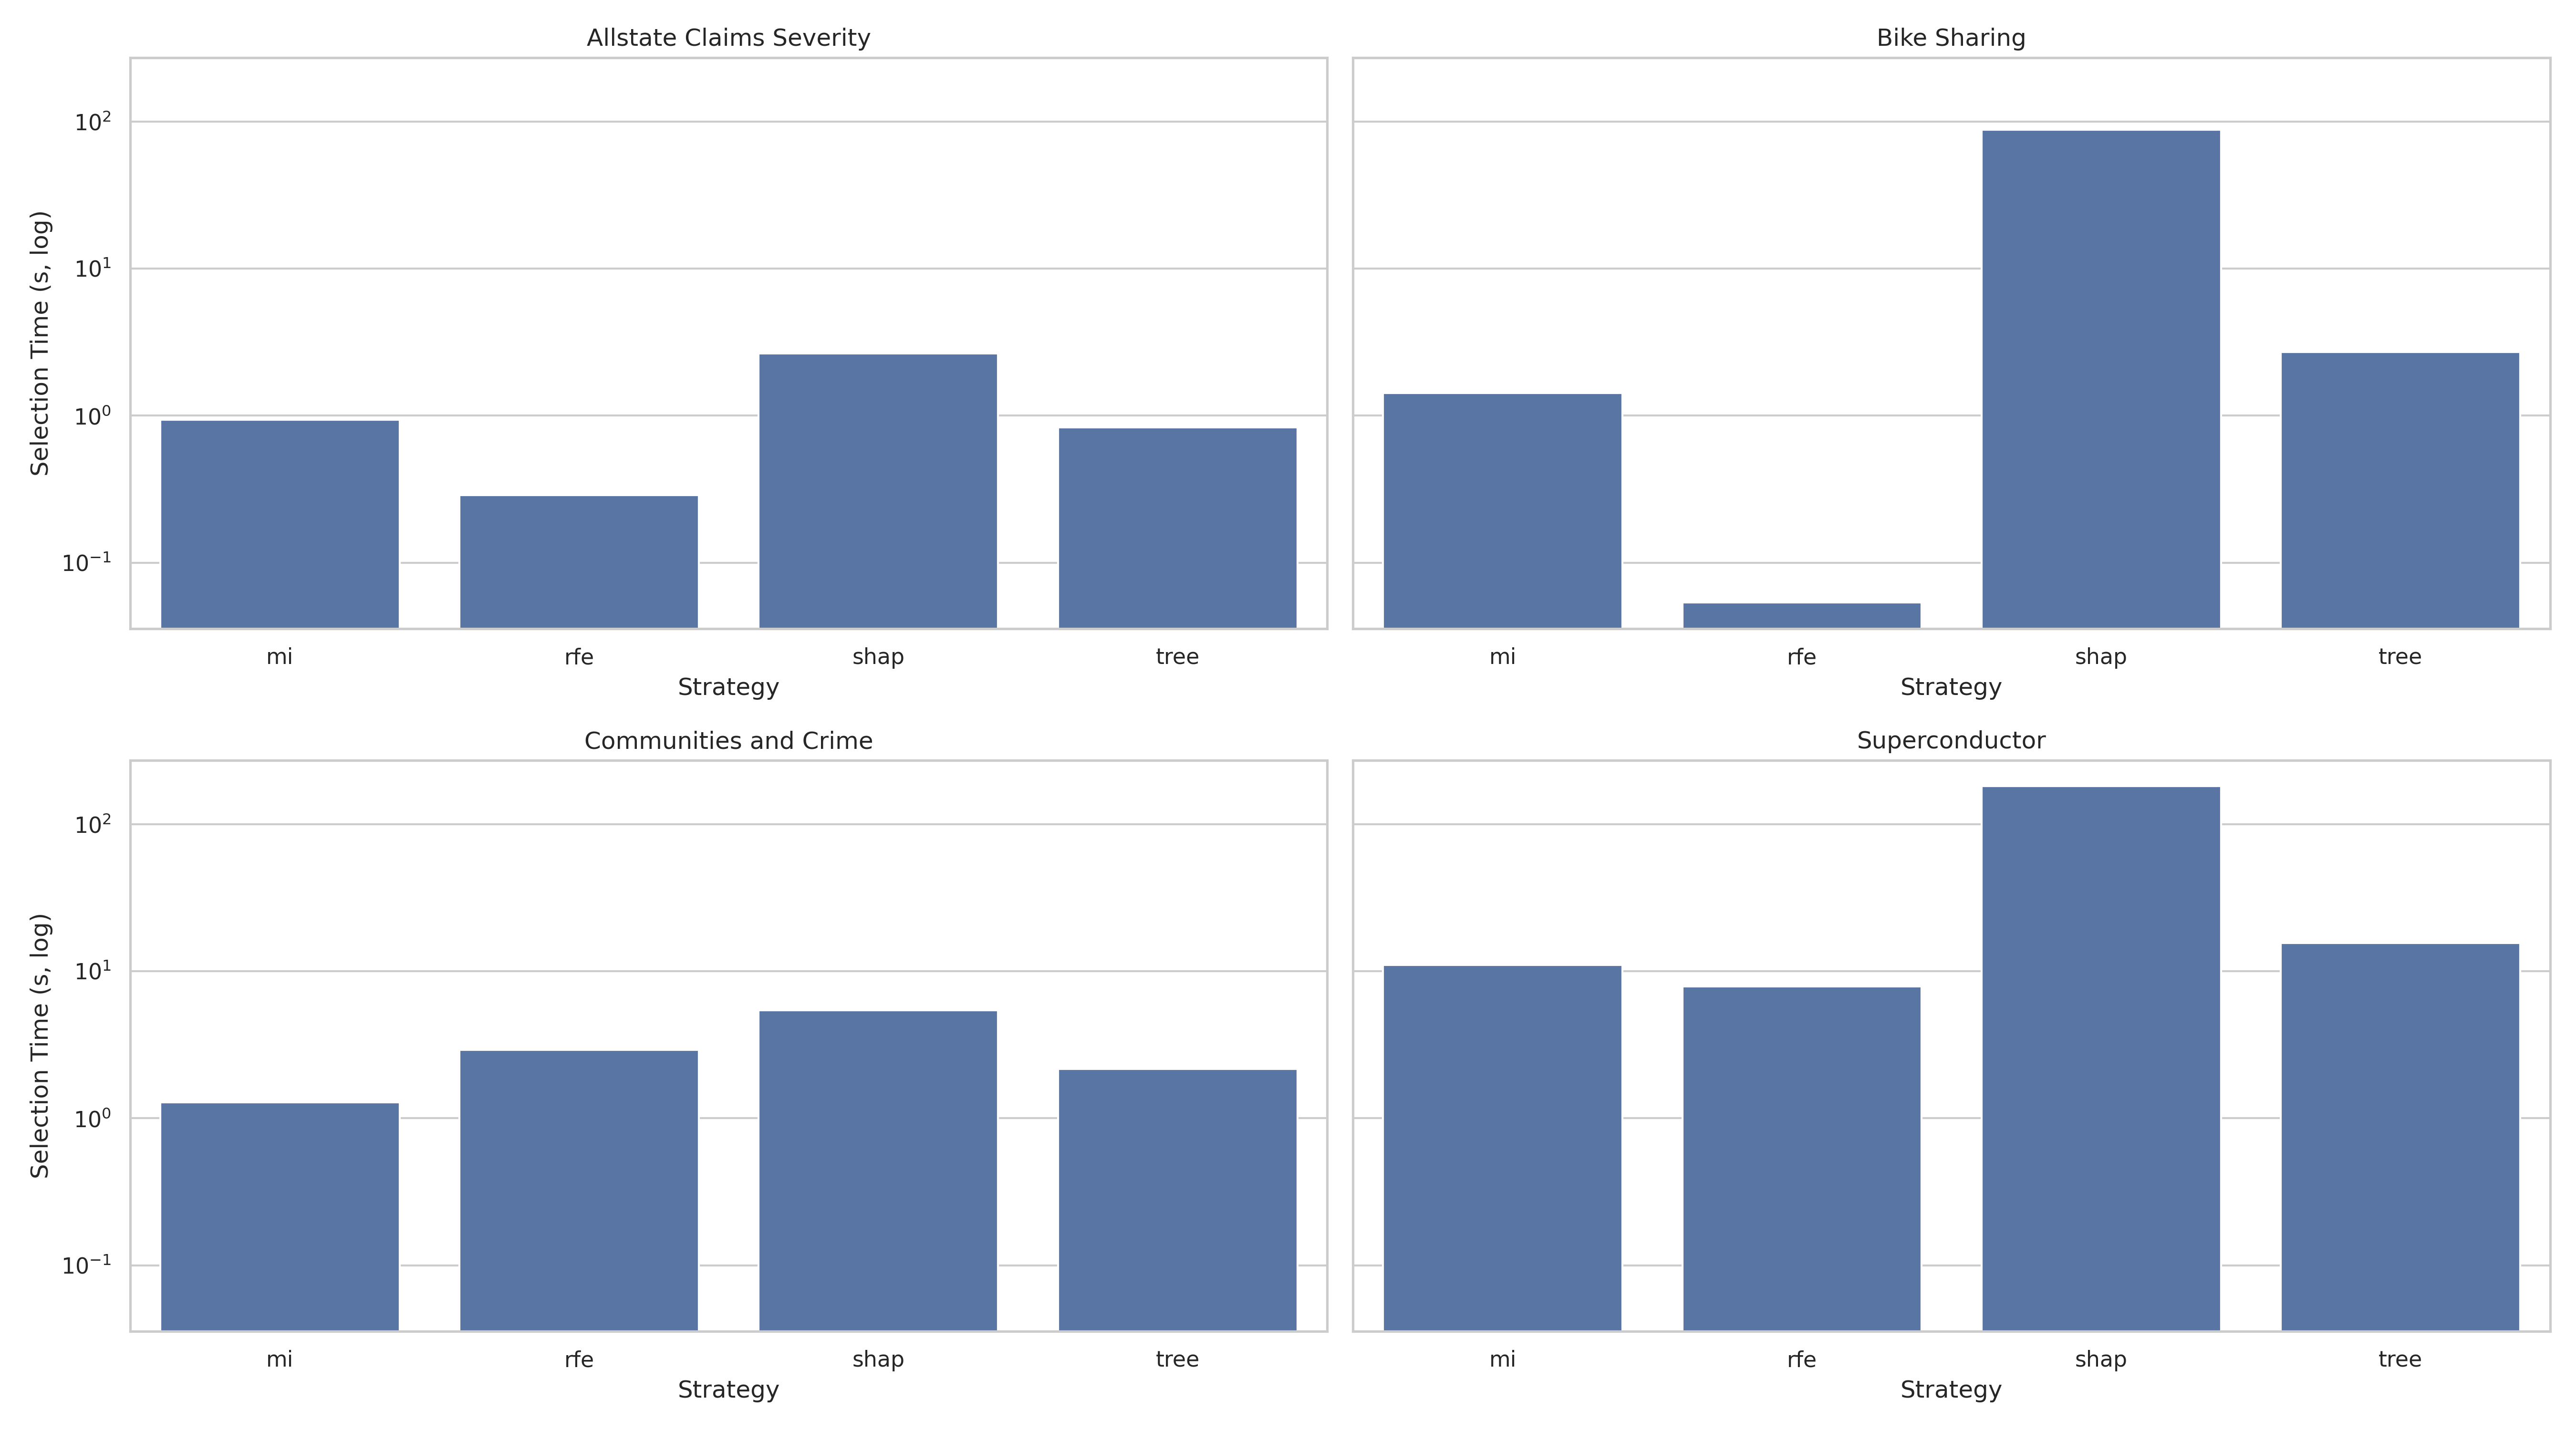
\includegraphics[width=0.85\textwidth]{../runs/exp1_plus_big-arff-run/figures/fig3_compute_cost_all_2x2.png}
    \caption{Stage~1 computational cost by strategy and dataset.}
    \label{fig:stage1_cost}
\end{figure}

\subsection{Selection Stability}

Table~\ref{tab:stage1_stability} summarizes Jaccard stability scores by strategy and retention level, averaged across datasets.

\begin{table}[h]
\centering
\caption{Mean Jaccard stability by strategy and retention level in Stage~1.}
\label{tab:stage1_stability}
\begin{tabular}{lrrrr}
\toprule
\textbf{Strategy} & \textbf{k=0.25} & \textbf{k=0.50} & \textbf{k=0.75} & \textbf{k=1.00} \\
\midrule
MI & 0.81 & 0.83 & 0.96 & 1.00 \\
RFE & 0.73 & 0.79 & 1.00 & 1.00 \\
SHAP & 0.63 & 0.77 & 0.97 & 1.00 \\
Tree-FI & 0.75 & 0.87 & 0.95 & 1.00 \\
\bottomrule
\end{tabular}
\end{table}

Stability increases with retention level across all methods, as expected---larger subsets have more overlap by construction. At $k=0.25$, SHAP shows the lowest stability (0.63), supporting hypothesis H4 that SHAP-based selection may introduce additional variability. By $k=0.75$, all methods converge to high stability.

\subsection{Stage 1 Summary}

The broad screening confirms that SHAP-based selection can be competitive but is not systematically superior. XGBoost emerges as the most consistent performer among models, making it the natural choice for the focused Stage~2 analysis. The computational overhead of SHAP depends heavily on the model family, with TreeExplainer providing efficiency for gradient boosting.

\section{Stage 2: Focused Deep-Dive Results}

Stage~2 applies three feature selection strategies plus a baseline to XGBoost on two selected datasets: Superconductor and Allstate Claims. A finer retention grid ($k \in \{0.05, 0.10, 0.15, 0.25, 0.50, 1.00\}$) enables more detailed analysis.

\subsection{Superconductor Dataset}

Table~\ref{tab:stage2_super} presents RMSE and total time for each strategy and retention level on the Superconductor dataset.

\begin{table}[h]
\centering
\caption{Superconductor results: RMSE and total time by strategy and retention level.}
\label{tab:stage2_super}
\begin{tabular}{llrr}
\toprule
\textbf{Strategy} & \textbf{k} & \textbf{RMSE} & \textbf{Time (s)} \\
\midrule
native\_fi & 0.05 & 13.44 & 4.02 \\
custom\_shap\_rfe & 0.05 & 13.48 & 3.99 \\
hybrid & 0.05 & 13.51 & 98.18 \\
\midrule
native\_fi & 0.10 & 11.20 & 4.07 \\
custom\_shap\_rfe & 0.10 & 11.10 & 4.02 \\
hybrid & 0.10 & 11.15 & 100.79 \\
\midrule
native\_fi & 0.25 & 10.30 & 4.19 \\
custom\_shap\_rfe & 0.25 & 10.35 & 4.14 \\
hybrid & 0.25 & 10.34 & 111.08 \\
\midrule
native\_fi & 0.50 & 10.08 & 4.29 \\
custom\_shap\_rfe & 0.50 & 10.06 & 4.28 \\
hybrid & 0.50 & 10.05 & 130.76 \\
\midrule
baseline & 1.00 & 9.94 & 4.51 \\
\bottomrule
\end{tabular}
\end{table}

Key observations:

\textbf{Baseline wins at full retention}: The best absolute RMSE (9.94) is achieved with all features retained, suggesting that for this dataset, feature selection does not improve over the full model.

\textbf{Marginal differences between selection strategies}: At each retention level, native\_fi, custom\_shap\_rfe, and hybrid produce nearly identical RMSE (differences $<0.1$). The sophisticated SHAP-based approaches do not outperform simple native importance.

\textbf{Dramatic cost difference}: The hybrid strategy requires 25-30x more time than native\_fi or custom\_shap\_rfe at comparable retention levels. For a $<0.1$ RMSE difference that sometimes favors simpler methods, this overhead is difficult to justify.

Figure~\ref{fig:stage2_super} visualizes the RMSE-time trade-off.

\begin{figure}[h]
    \centering
    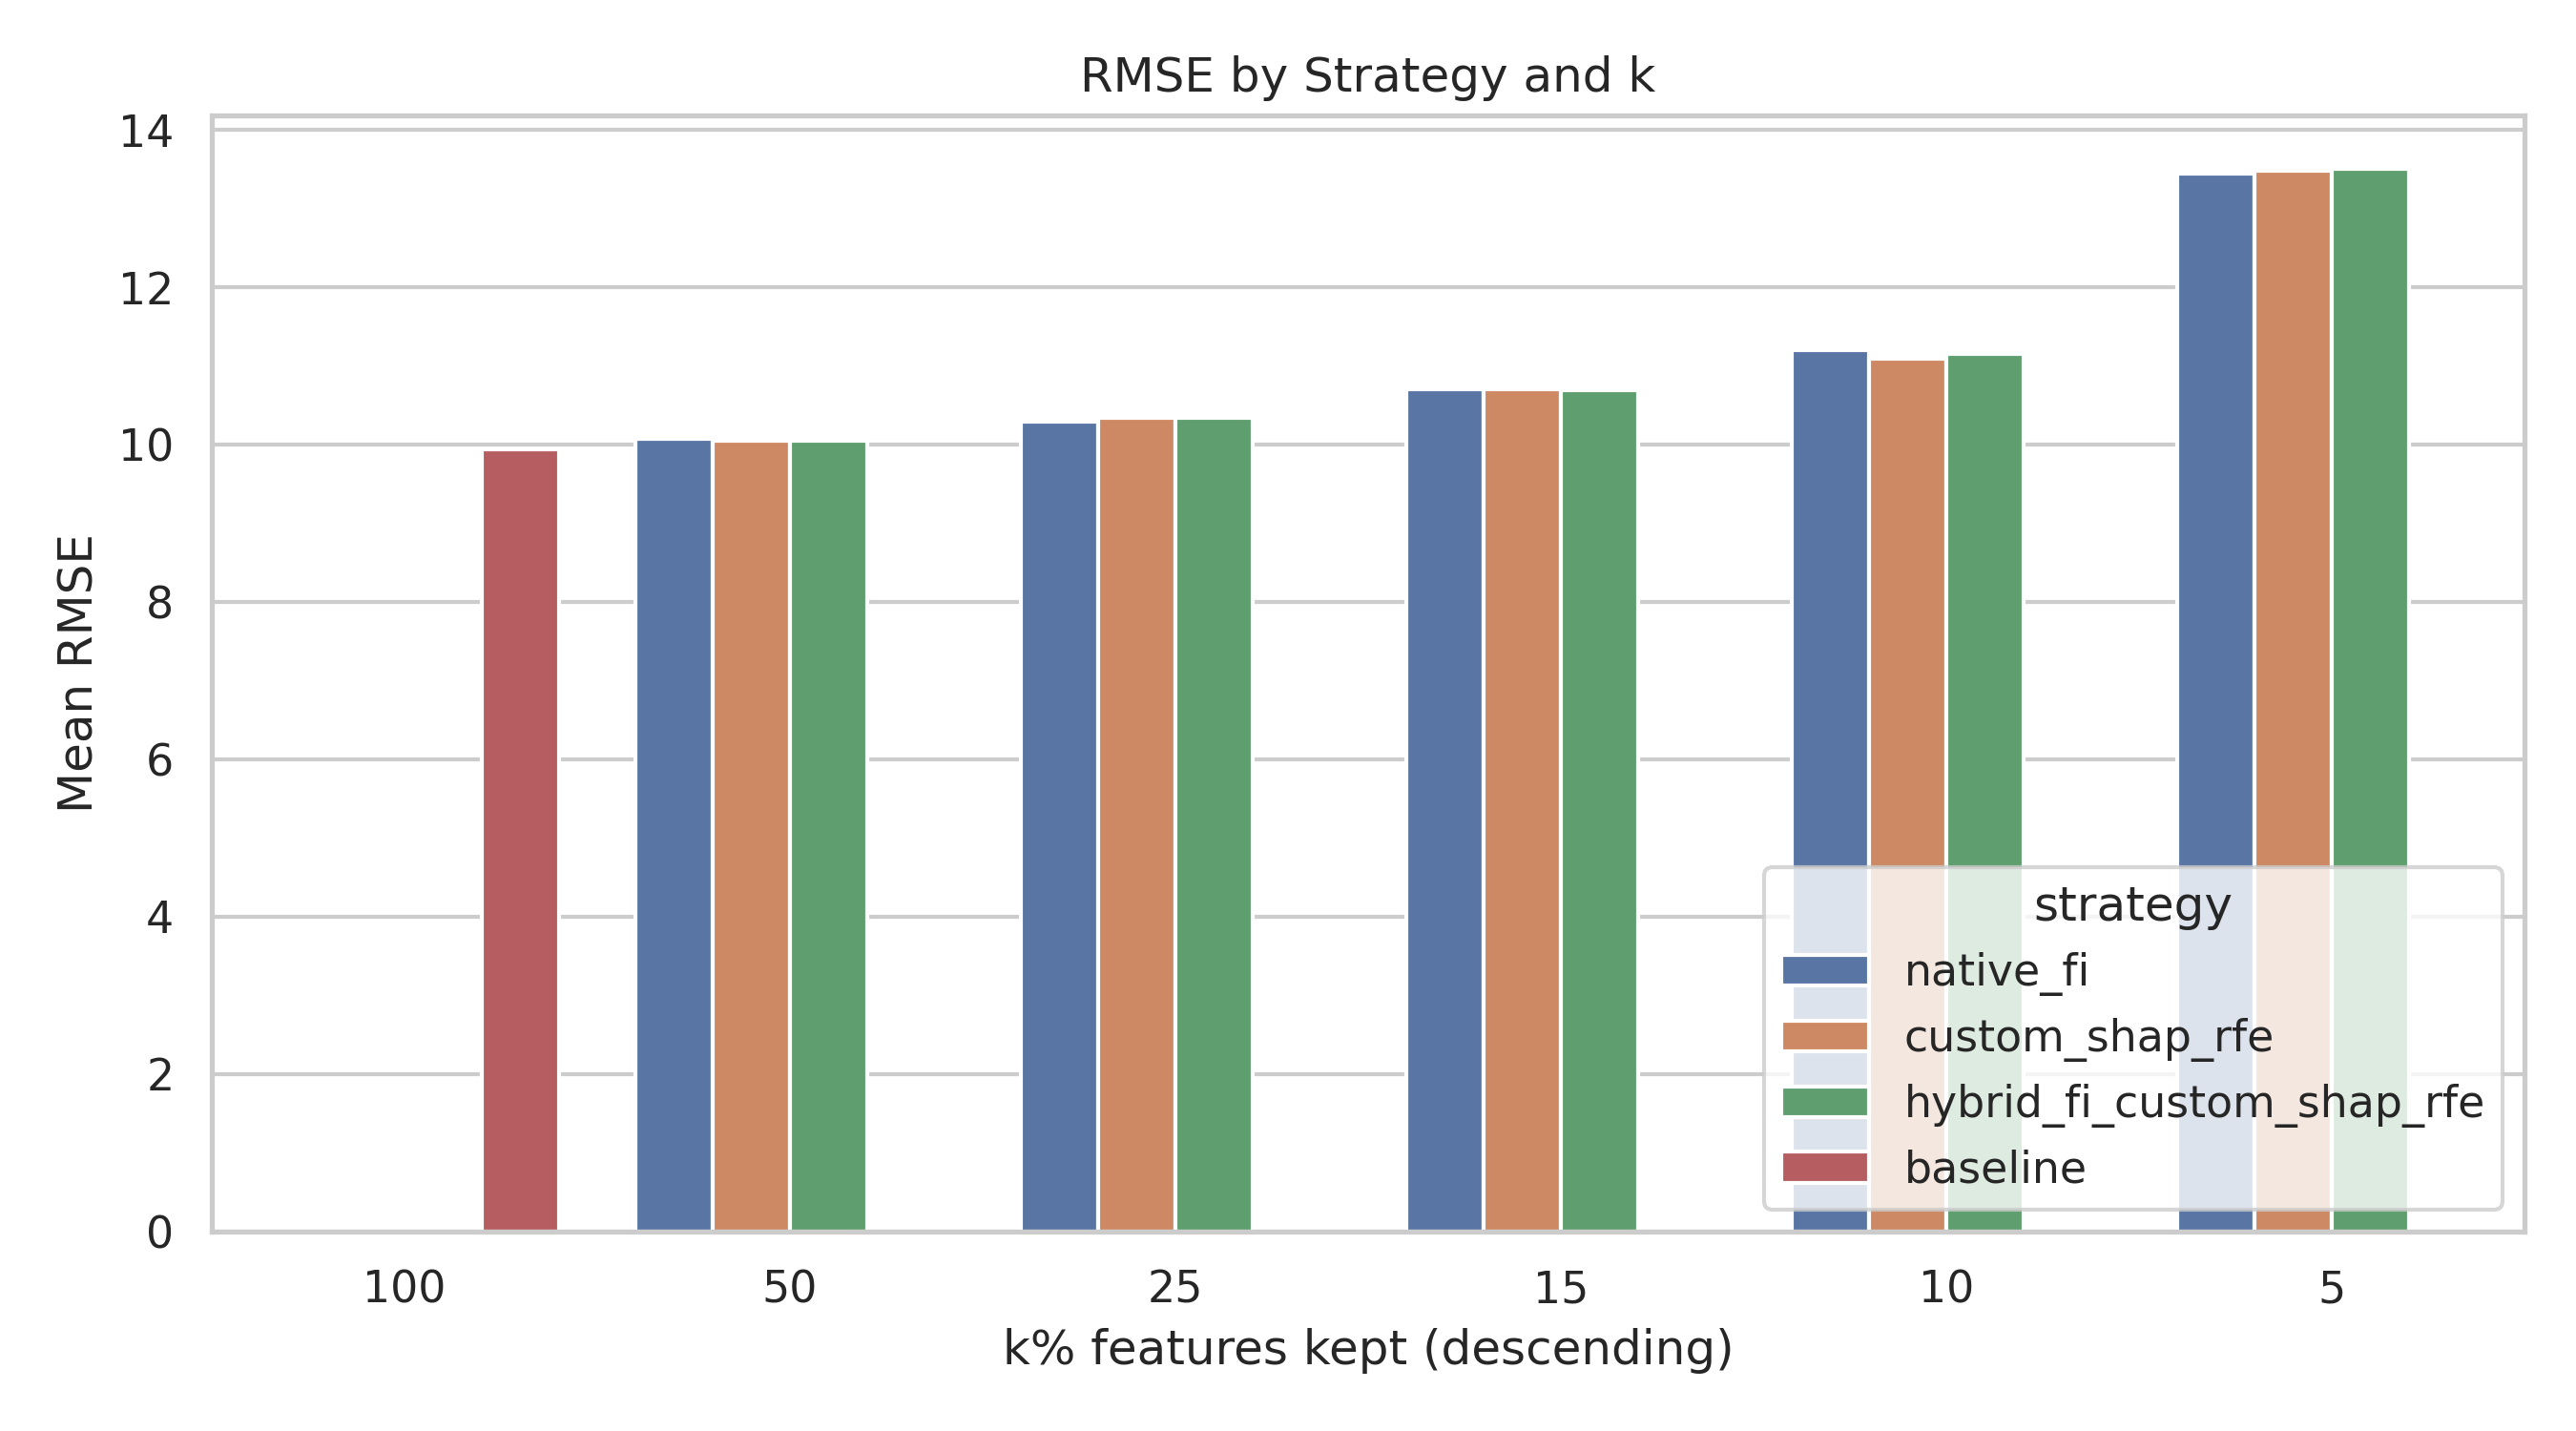
\includegraphics[width=0.48\textwidth]{../runs/exp2_run12/figures/exp2_rmse_by_strategy_k.png}
    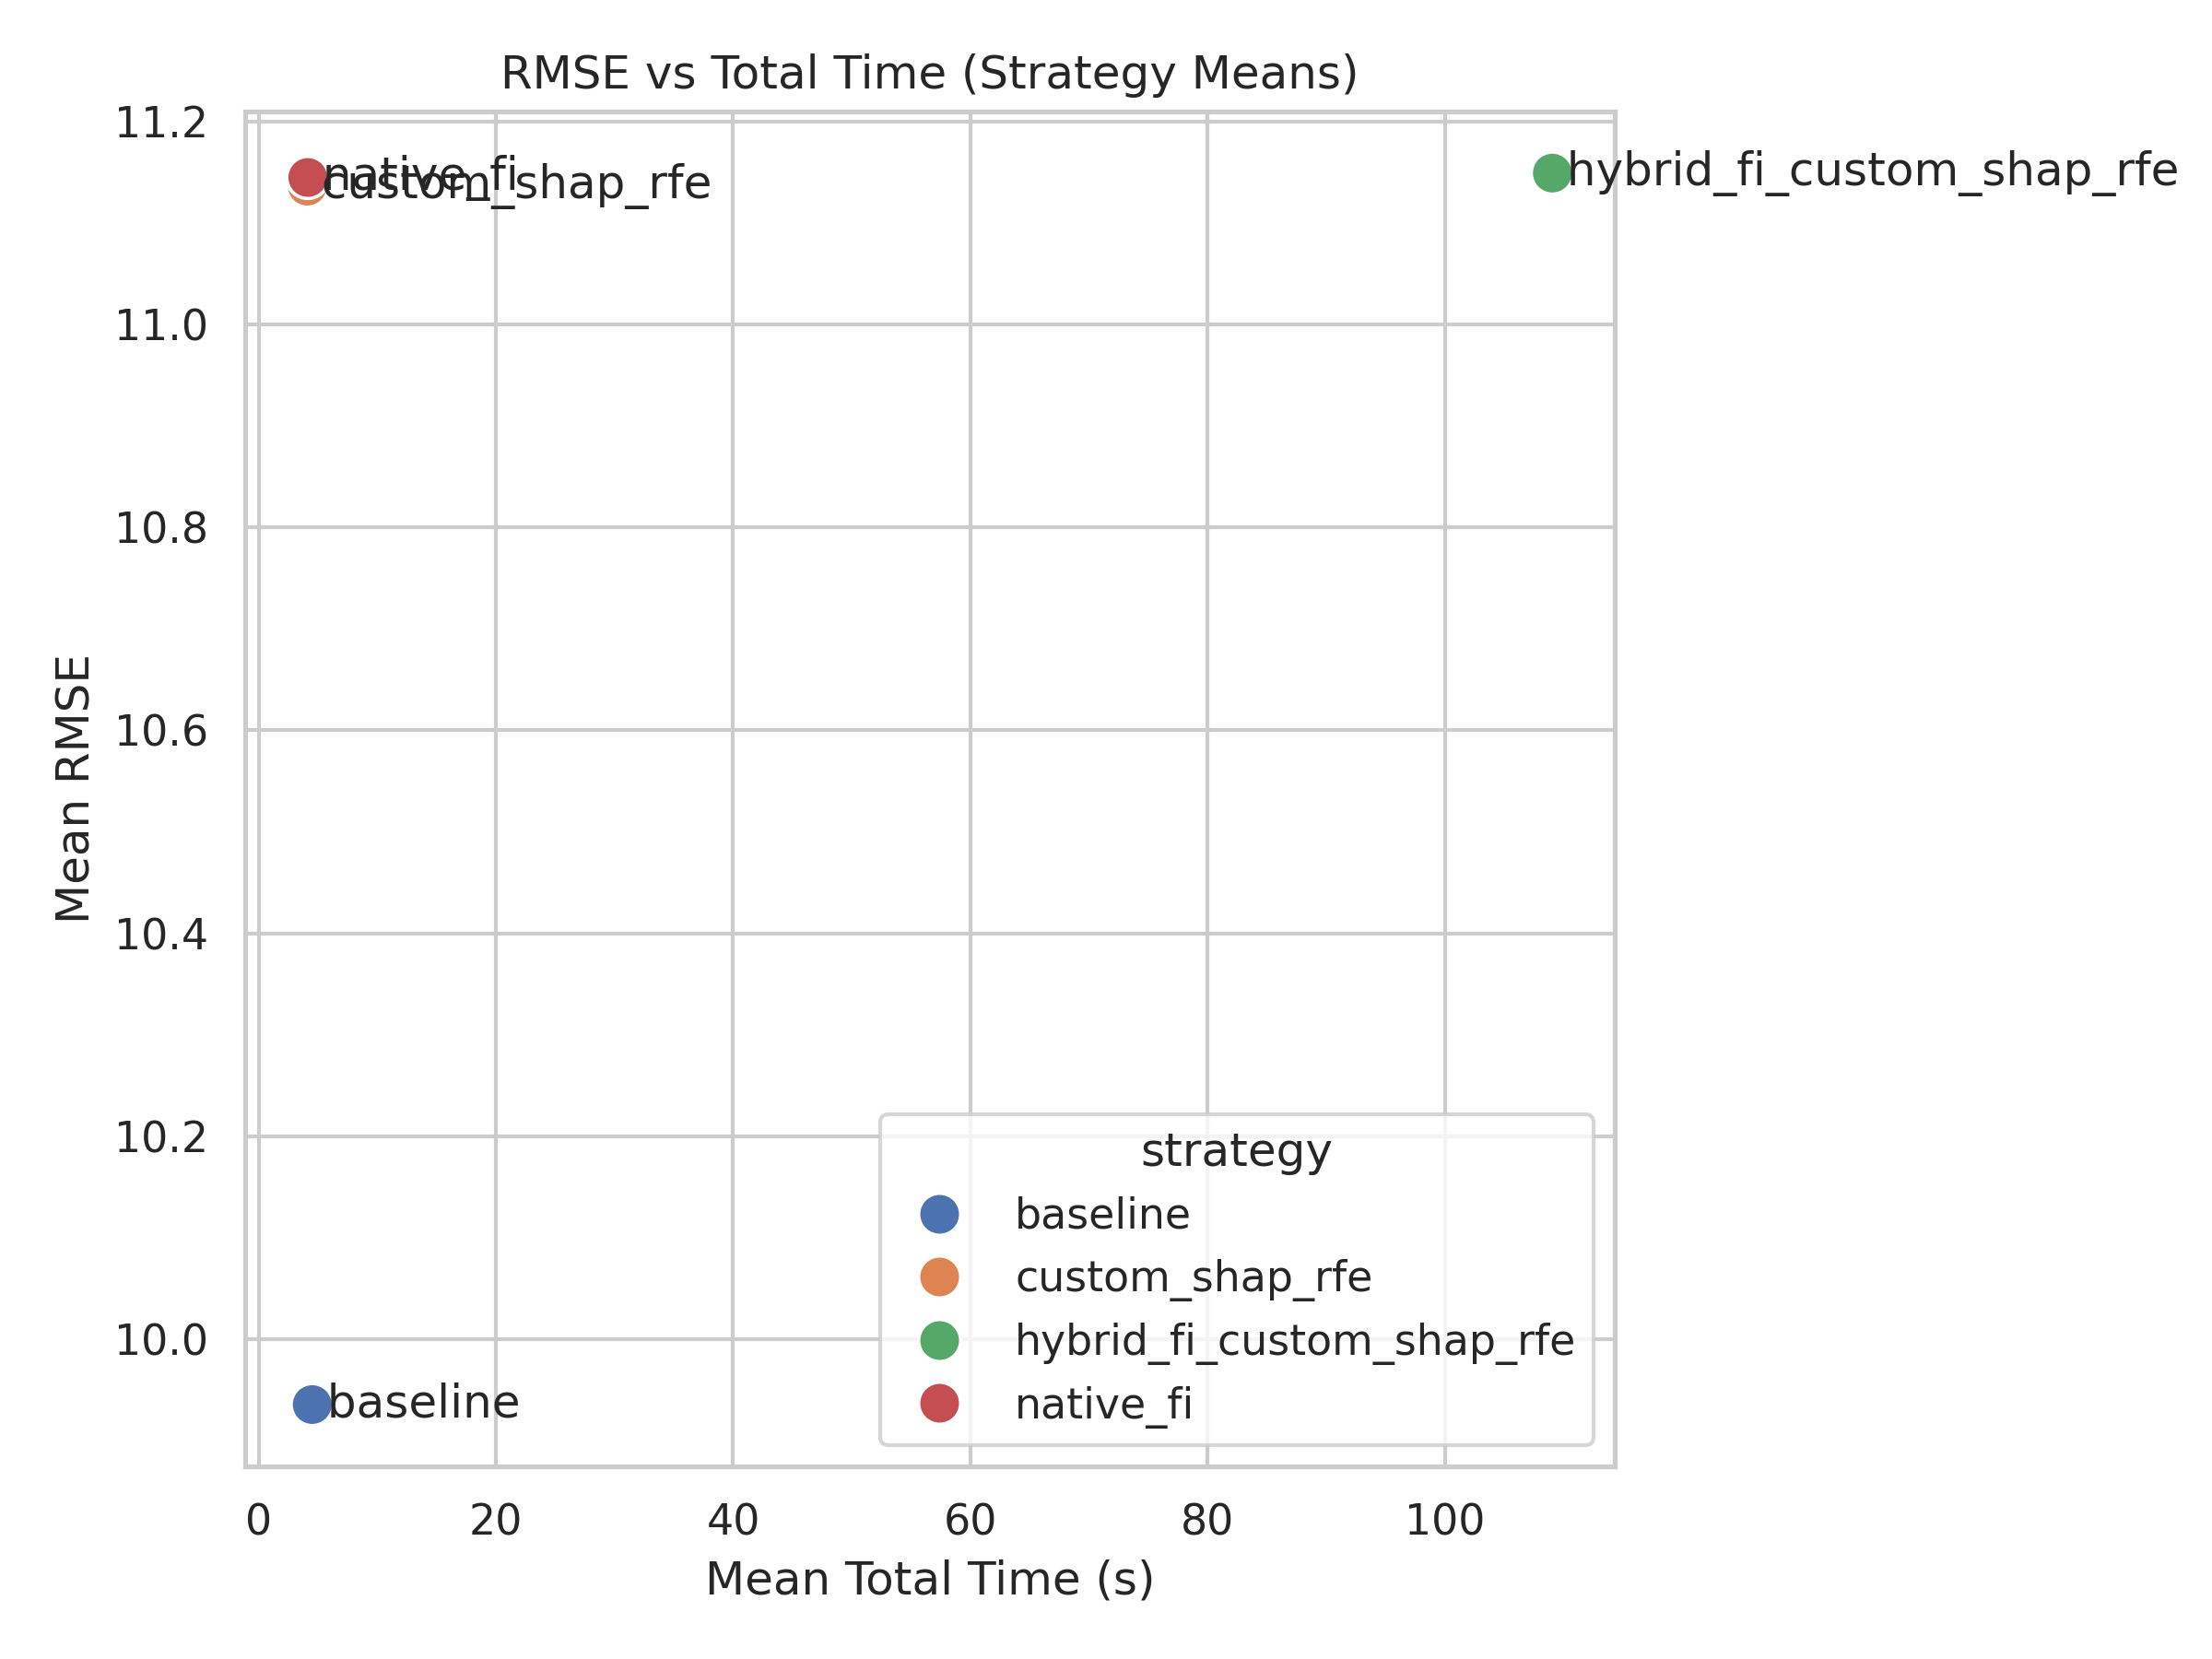
\includegraphics[width=0.48\textwidth]{../runs/exp2_run12/figures/exp2_rmse_vs_time_tradeoff.png}
    \caption{Superconductor deep-dive: RMSE by retention level (left) and RMSE vs. total time trade-off (right).}
    \label{fig:stage2_super}
\end{figure}

\subsection{Allstate Claims Dataset}

Table~\ref{tab:stage2_allstate} presents corresponding results for the Allstate dataset.

\begin{table}[h]
\centering
\caption{Allstate Claims results: RMSE and total time by strategy and retention level.}
\label{tab:stage2_allstate}
\begin{tabular}{llrr}
\toprule
\textbf{Strategy} & \textbf{k} & \textbf{RMSE} & \textbf{Time (s)} \\
\midrule
native\_fi & 0.05 & 2198.79 & 7.86 \\
custom\_shap\_rfe & 0.05 & 2277.81 & 7.52 \\
hybrid & 0.05 & 2224.63 & 129.69 \\
\midrule
native\_fi & 0.10 & 2062.39 & 7.96 \\
custom\_shap\_rfe & 0.10 & 2088.88 & 7.94 \\
hybrid & 0.10 & 2016.12 & 135.12 \\
\midrule
native\_fi & 0.25 & 1929.38 & 8.31 \\
custom\_shap\_rfe & 0.25 & 1925.70 & 8.50 \\
hybrid & 0.25 & 1932.26 & 152.25 \\
\midrule
native\_fi & 0.50 & 1912.92 & 8.93 \\
custom\_shap\_rfe & 0.50 & 1913.03 & 9.31 \\
hybrid & 0.50 & 1913.72 & 180.42 \\
\midrule
baseline & 1.00 & 1913.12 & 9.94 \\
\bottomrule
\end{tabular}
\end{table}

On Allstate, patterns are similar to Superconductor:

\textbf{Feature selection matches baseline}: At $k=0.50$, native\_fi achieves RMSE 1912.92, essentially identical to the baseline (1913.12). Selection provides no meaningful improvement.

\textbf{SHAP-RFE occasionally wins}: At $k=0.25$, custom\_shap\_rfe achieves the best RMSE (1925.70), marginally better than native\_fi (1929.38). This is consistent with hypothesis H2---small gains at intermediate retention.

\textbf{Hybrid underperforms and costs more}: At $k=0.50$, hybrid produces the worst RMSE (1913.72) among selection methods while requiring 20x more time than native\_fi.

Figure~\ref{fig:stage2_allstate} shows the trade-off visualization.

\begin{figure}[h]
    \centering
    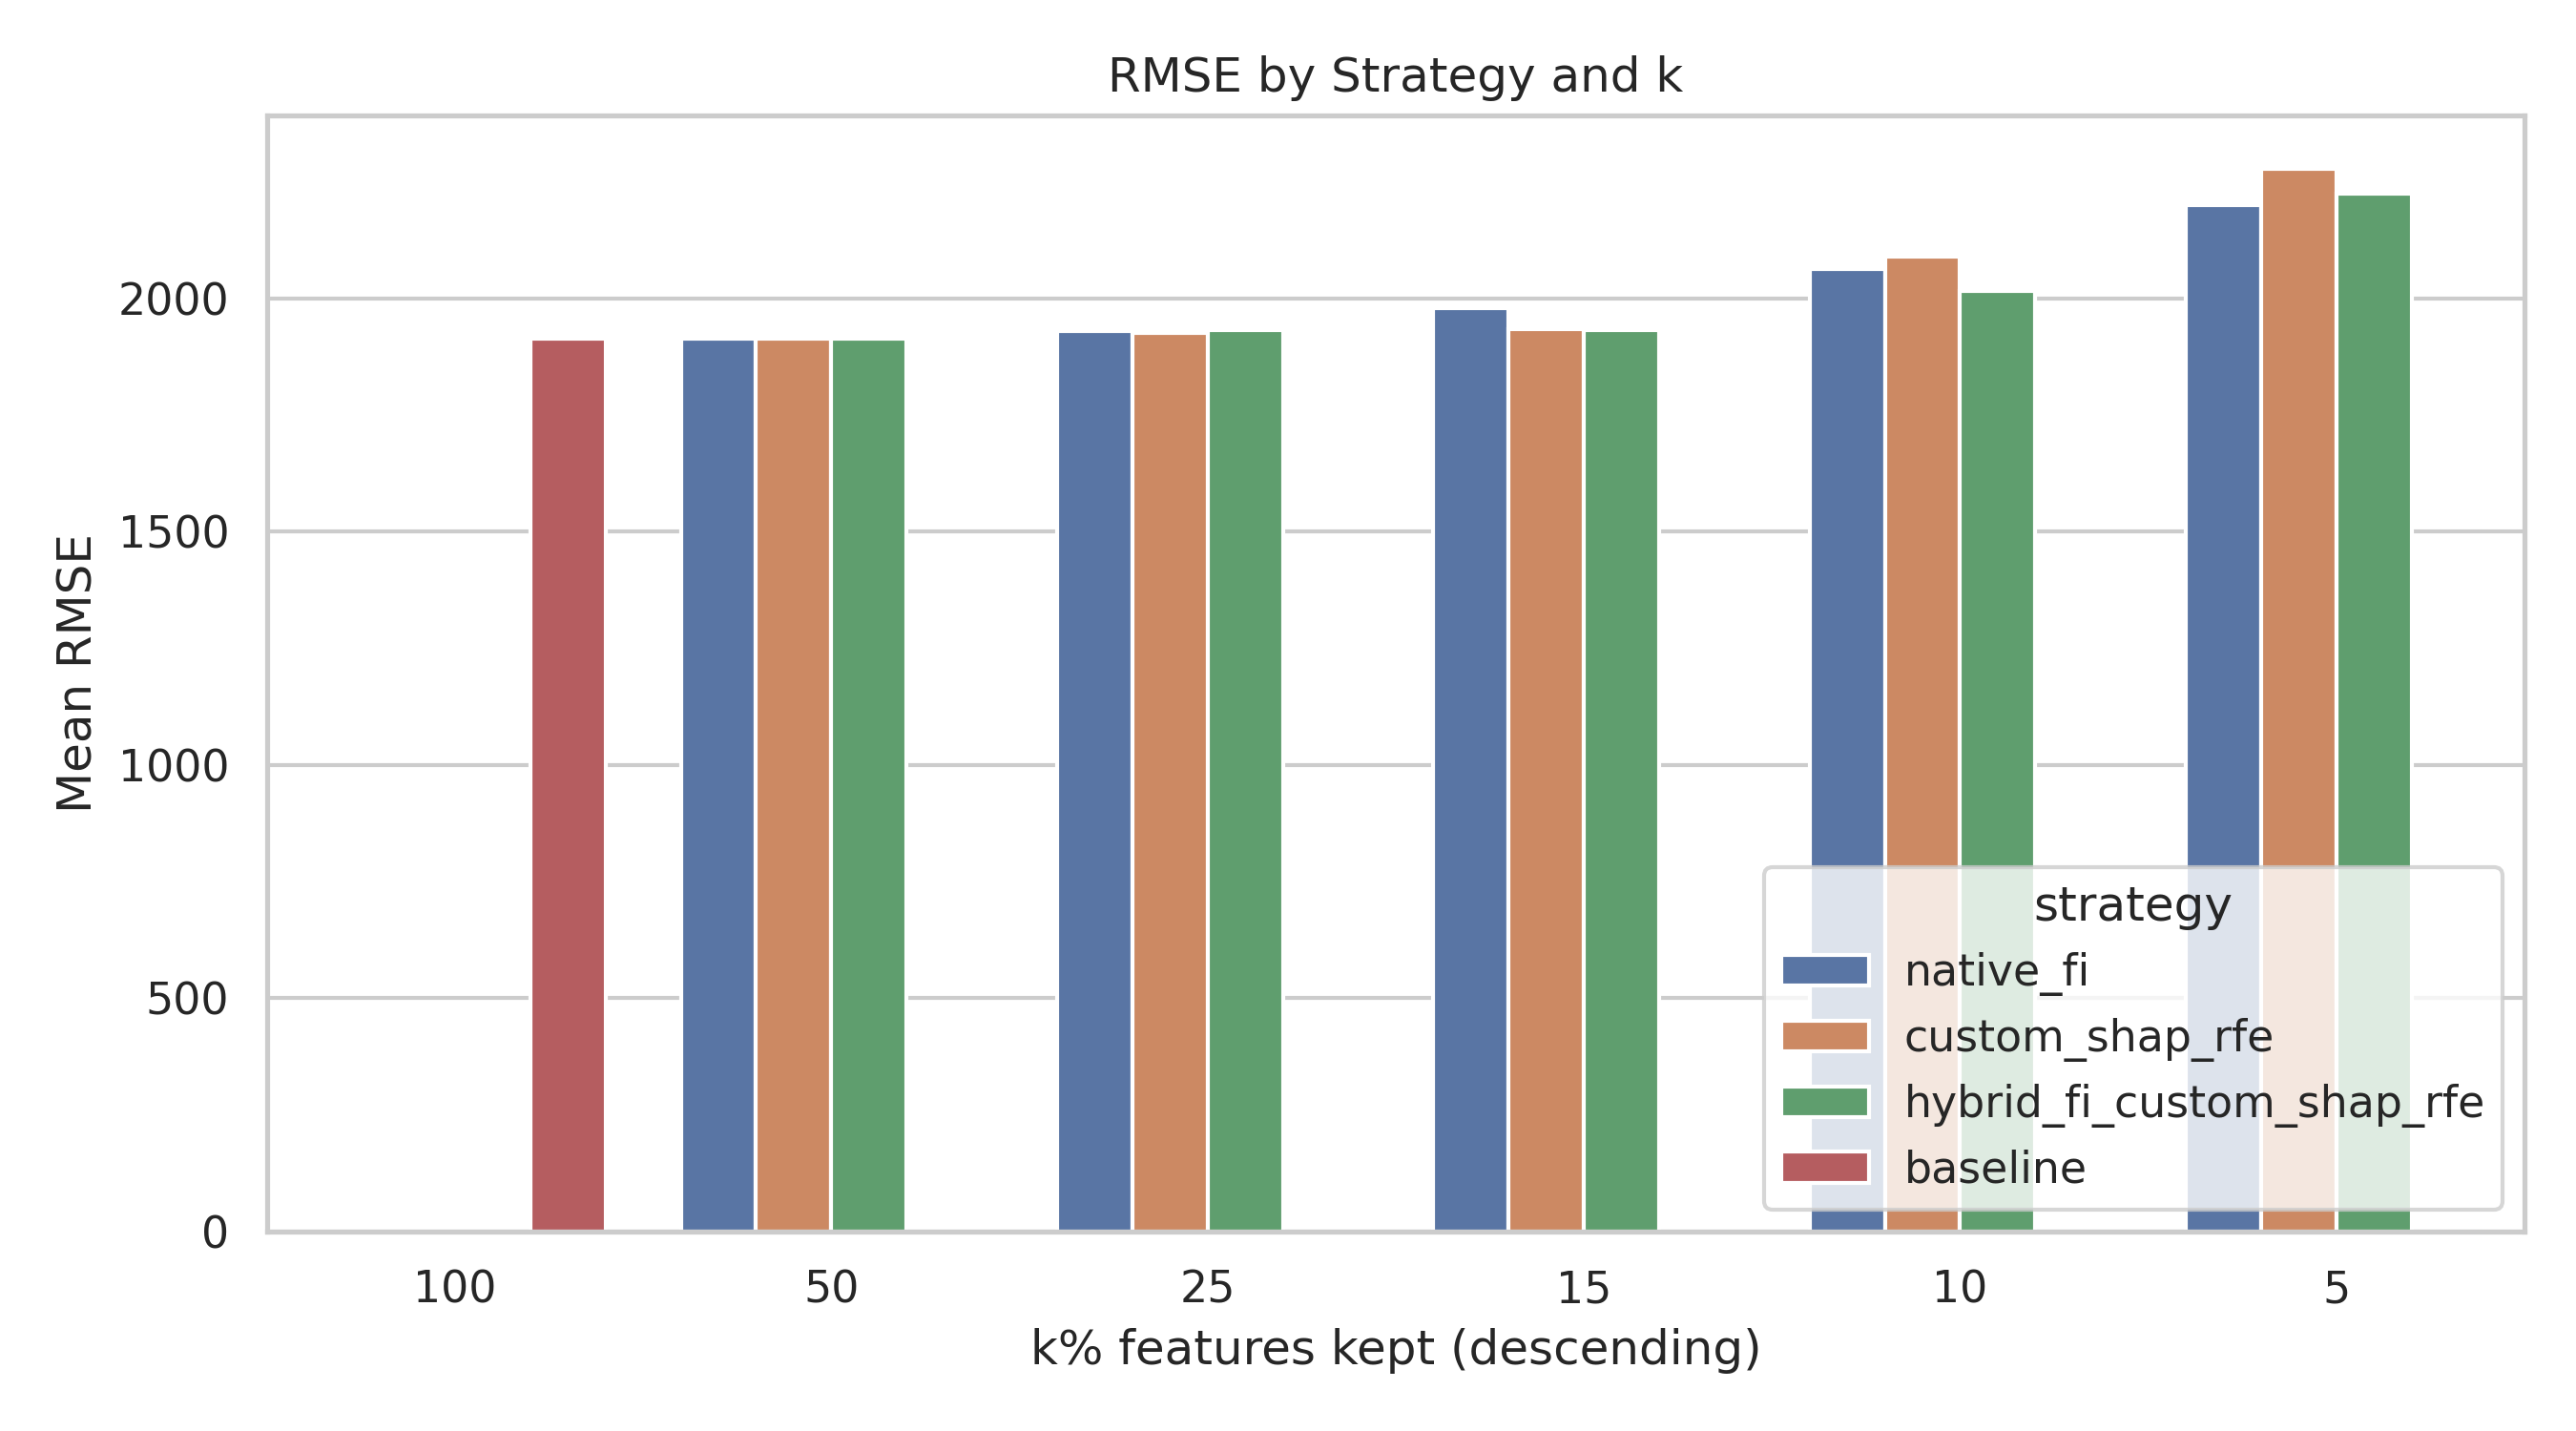
\includegraphics[width=0.48\textwidth]{../runs/exp3_run01/figures/exp3_rmse_by_strategy_k.png}
    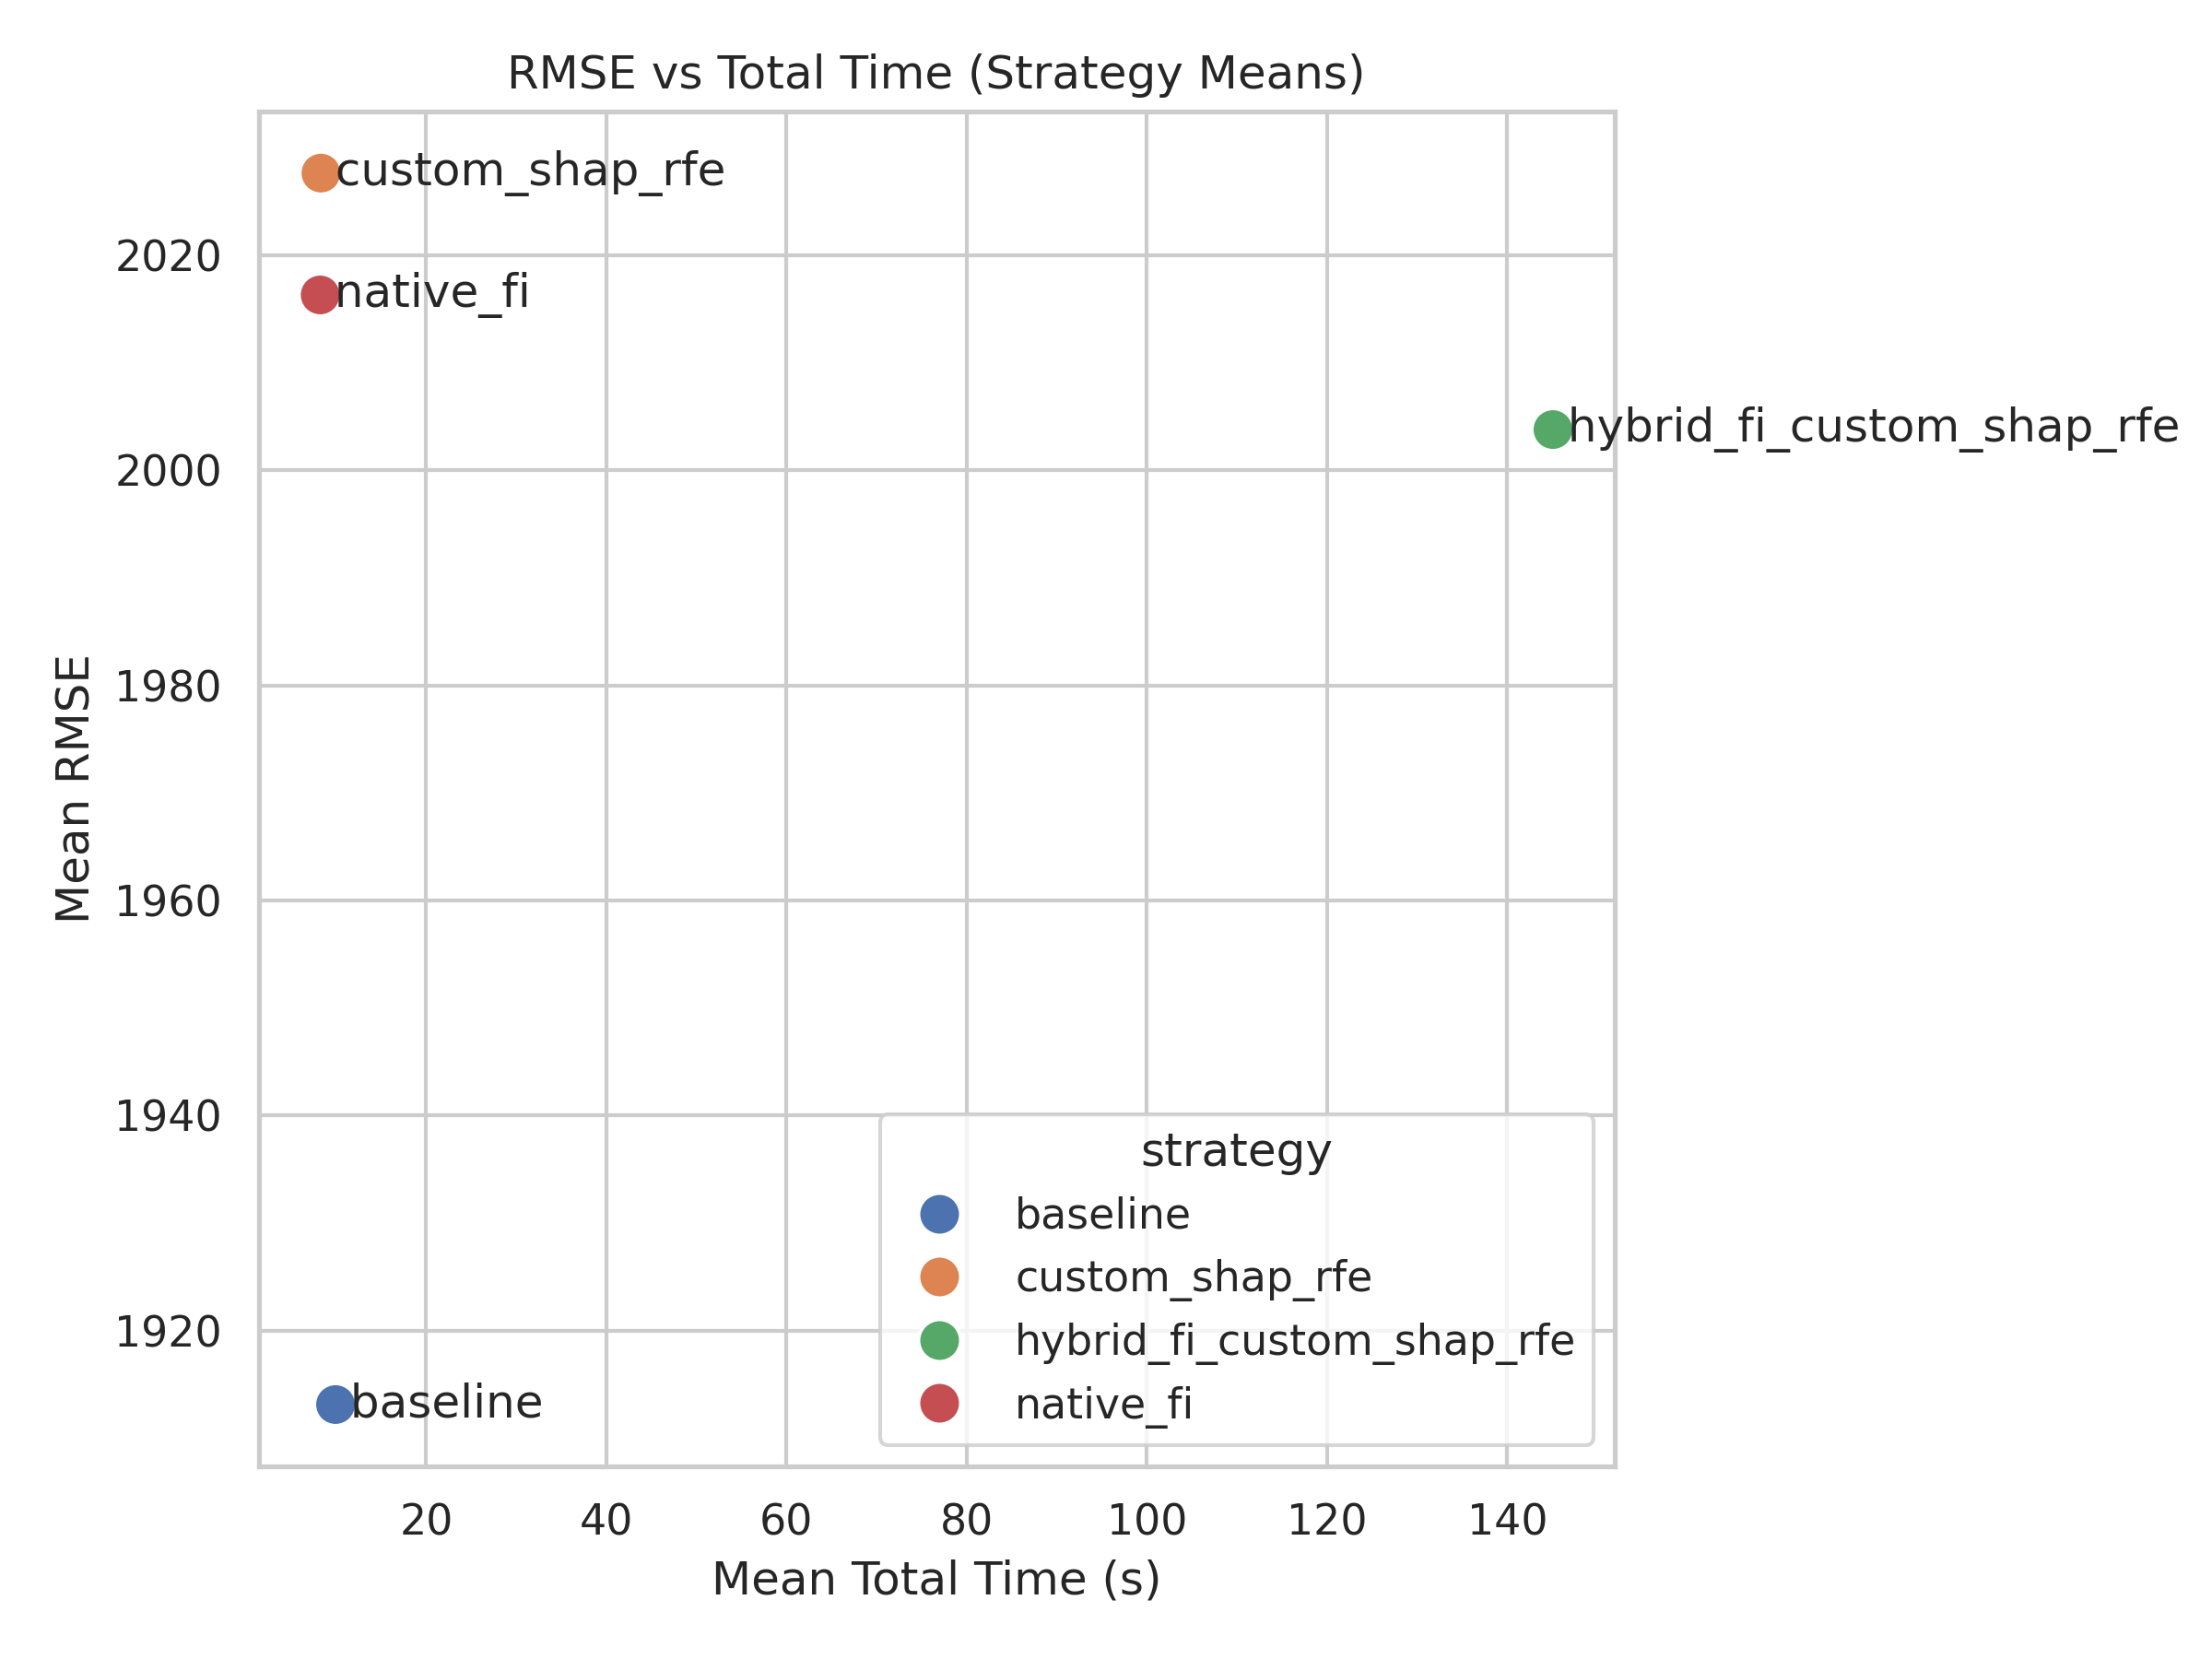
\includegraphics[width=0.48\textwidth]{../runs/exp3_run01/figures/exp3_rmse_vs_time_tradeoff.png}
    \caption{Allstate Claims deep-dive: RMSE by retention level (left) and RMSE vs. total time trade-off (right).}
    \label{fig:stage2_allstate}
\end{figure}

\subsection{Stability in Stage 2}

Figure~\ref{fig:stage2_stability} shows selection stability across retention levels for both datasets.

\begin{figure}[h]
    \centering
    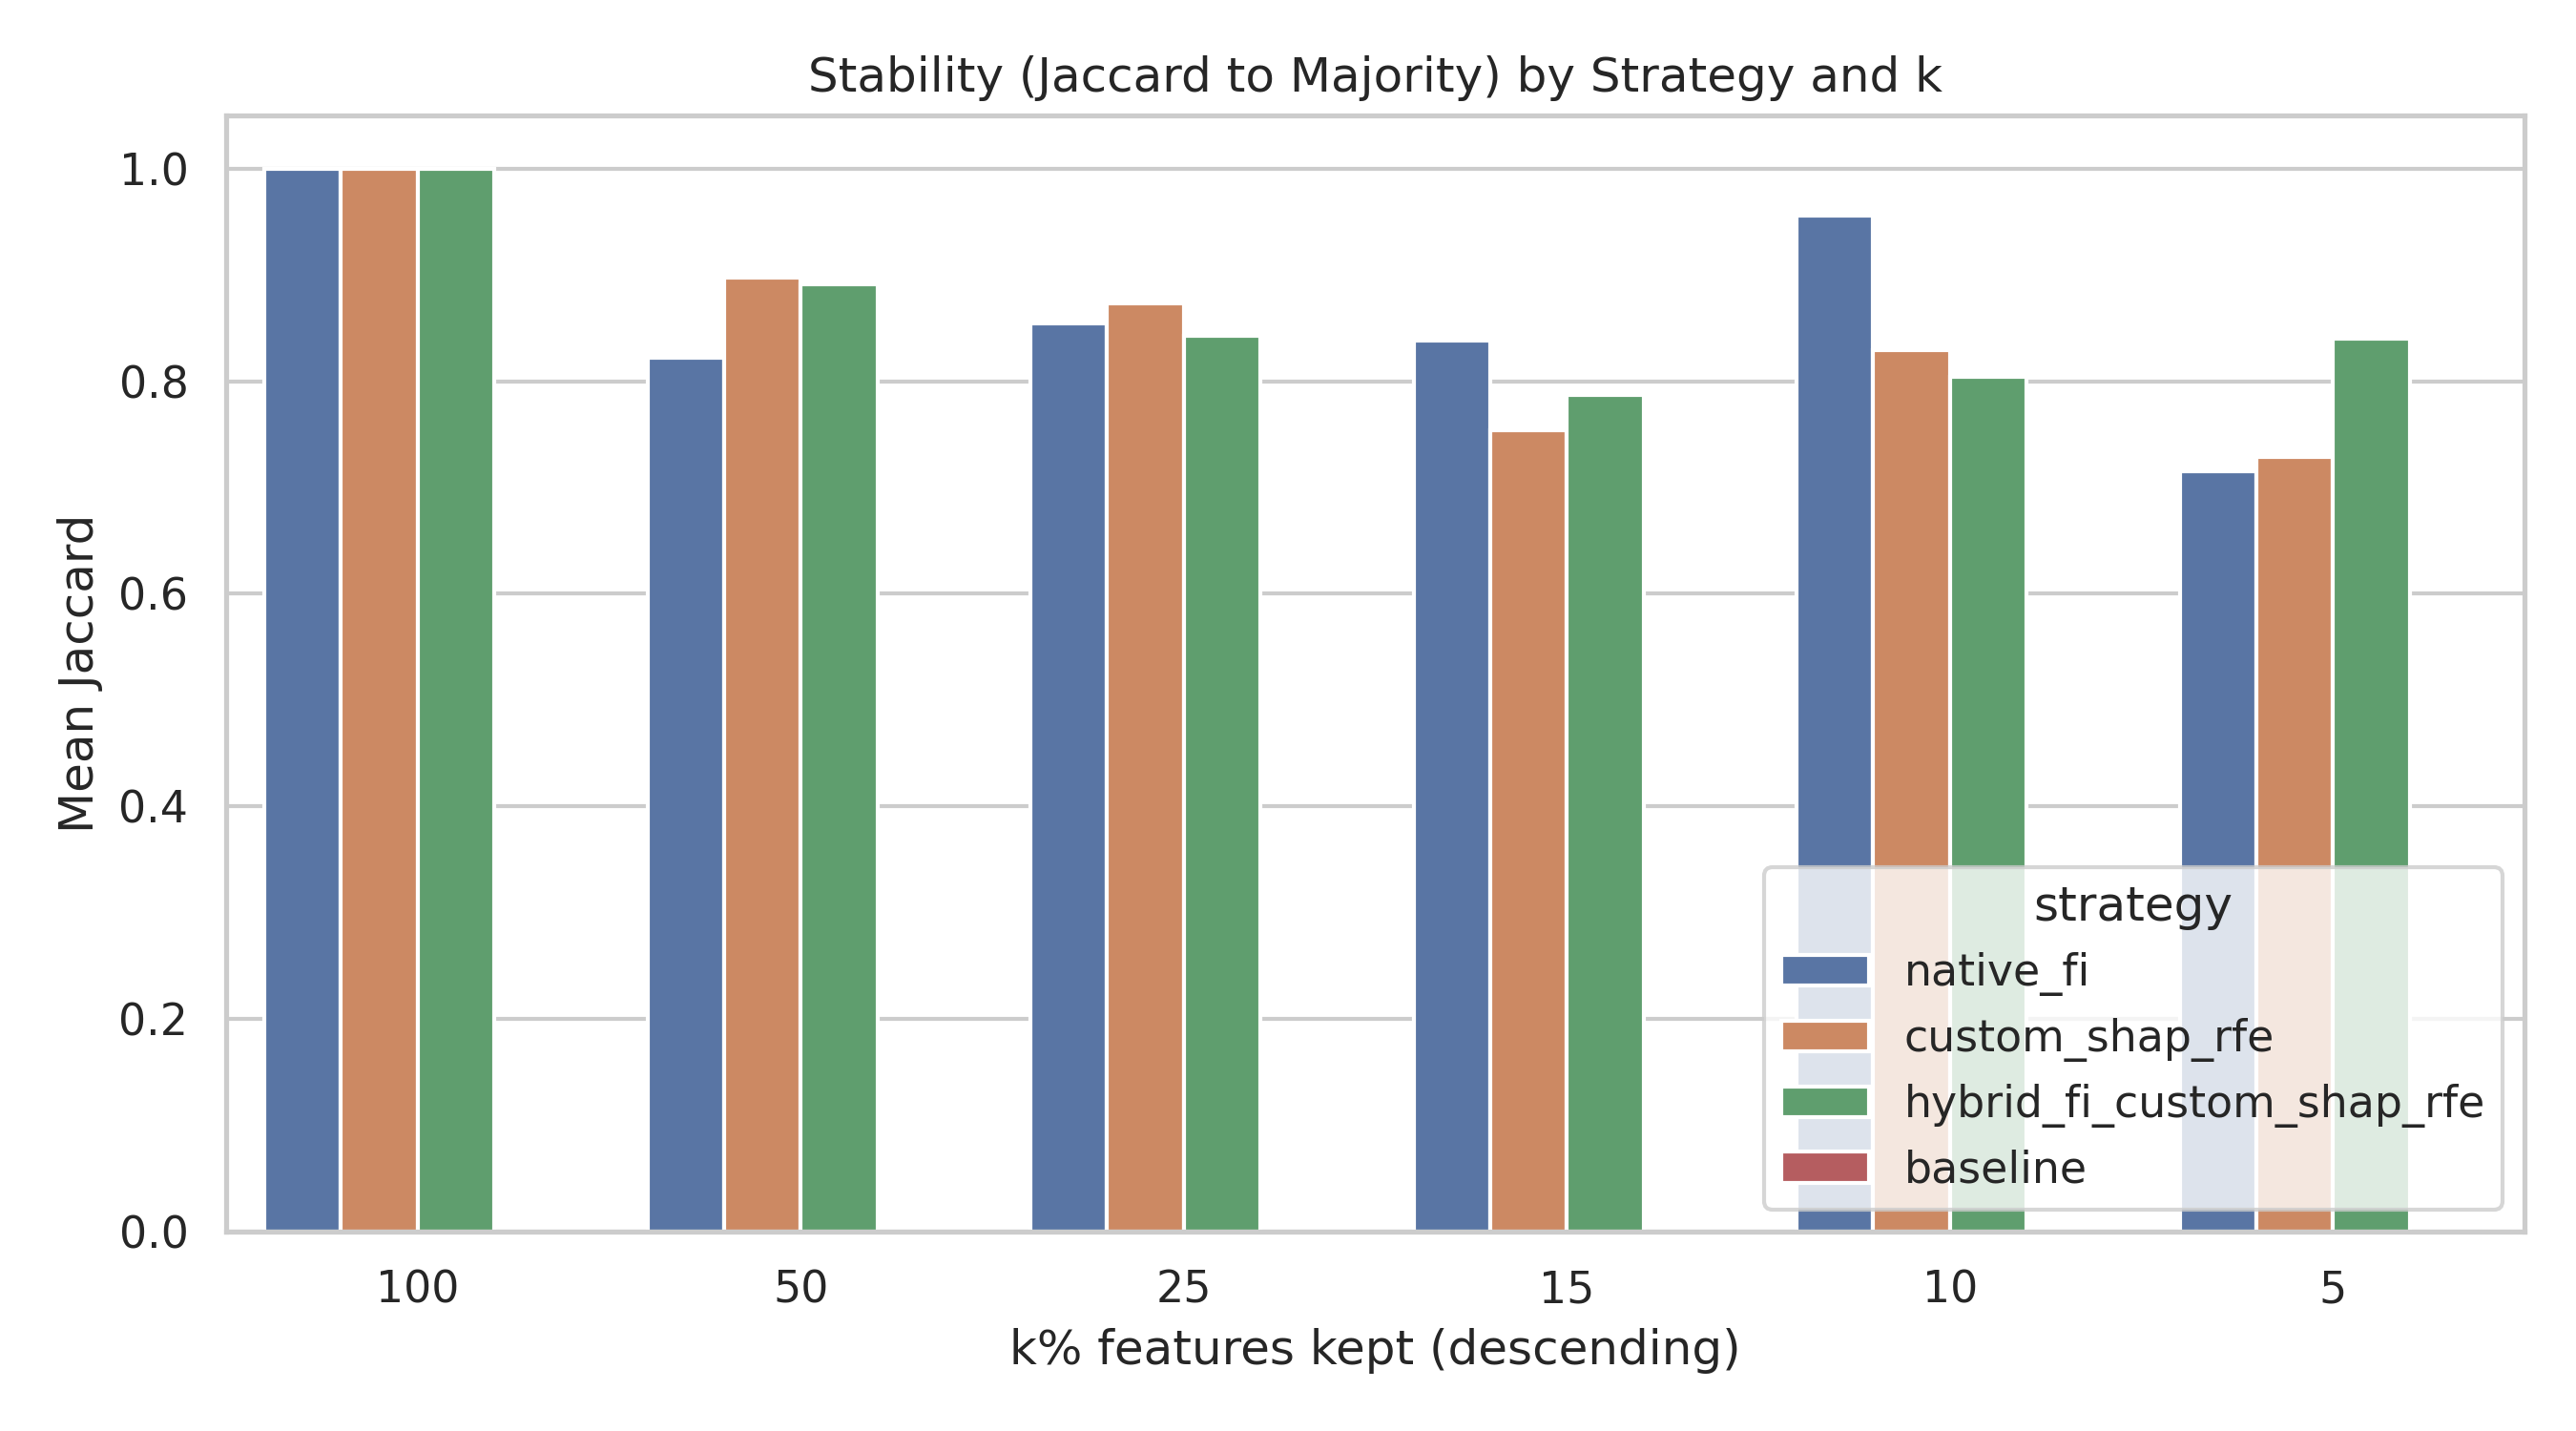
\includegraphics[width=0.48\textwidth]{../runs/exp2_run12/figures/exp2_stability_by_strategy_k.png}
    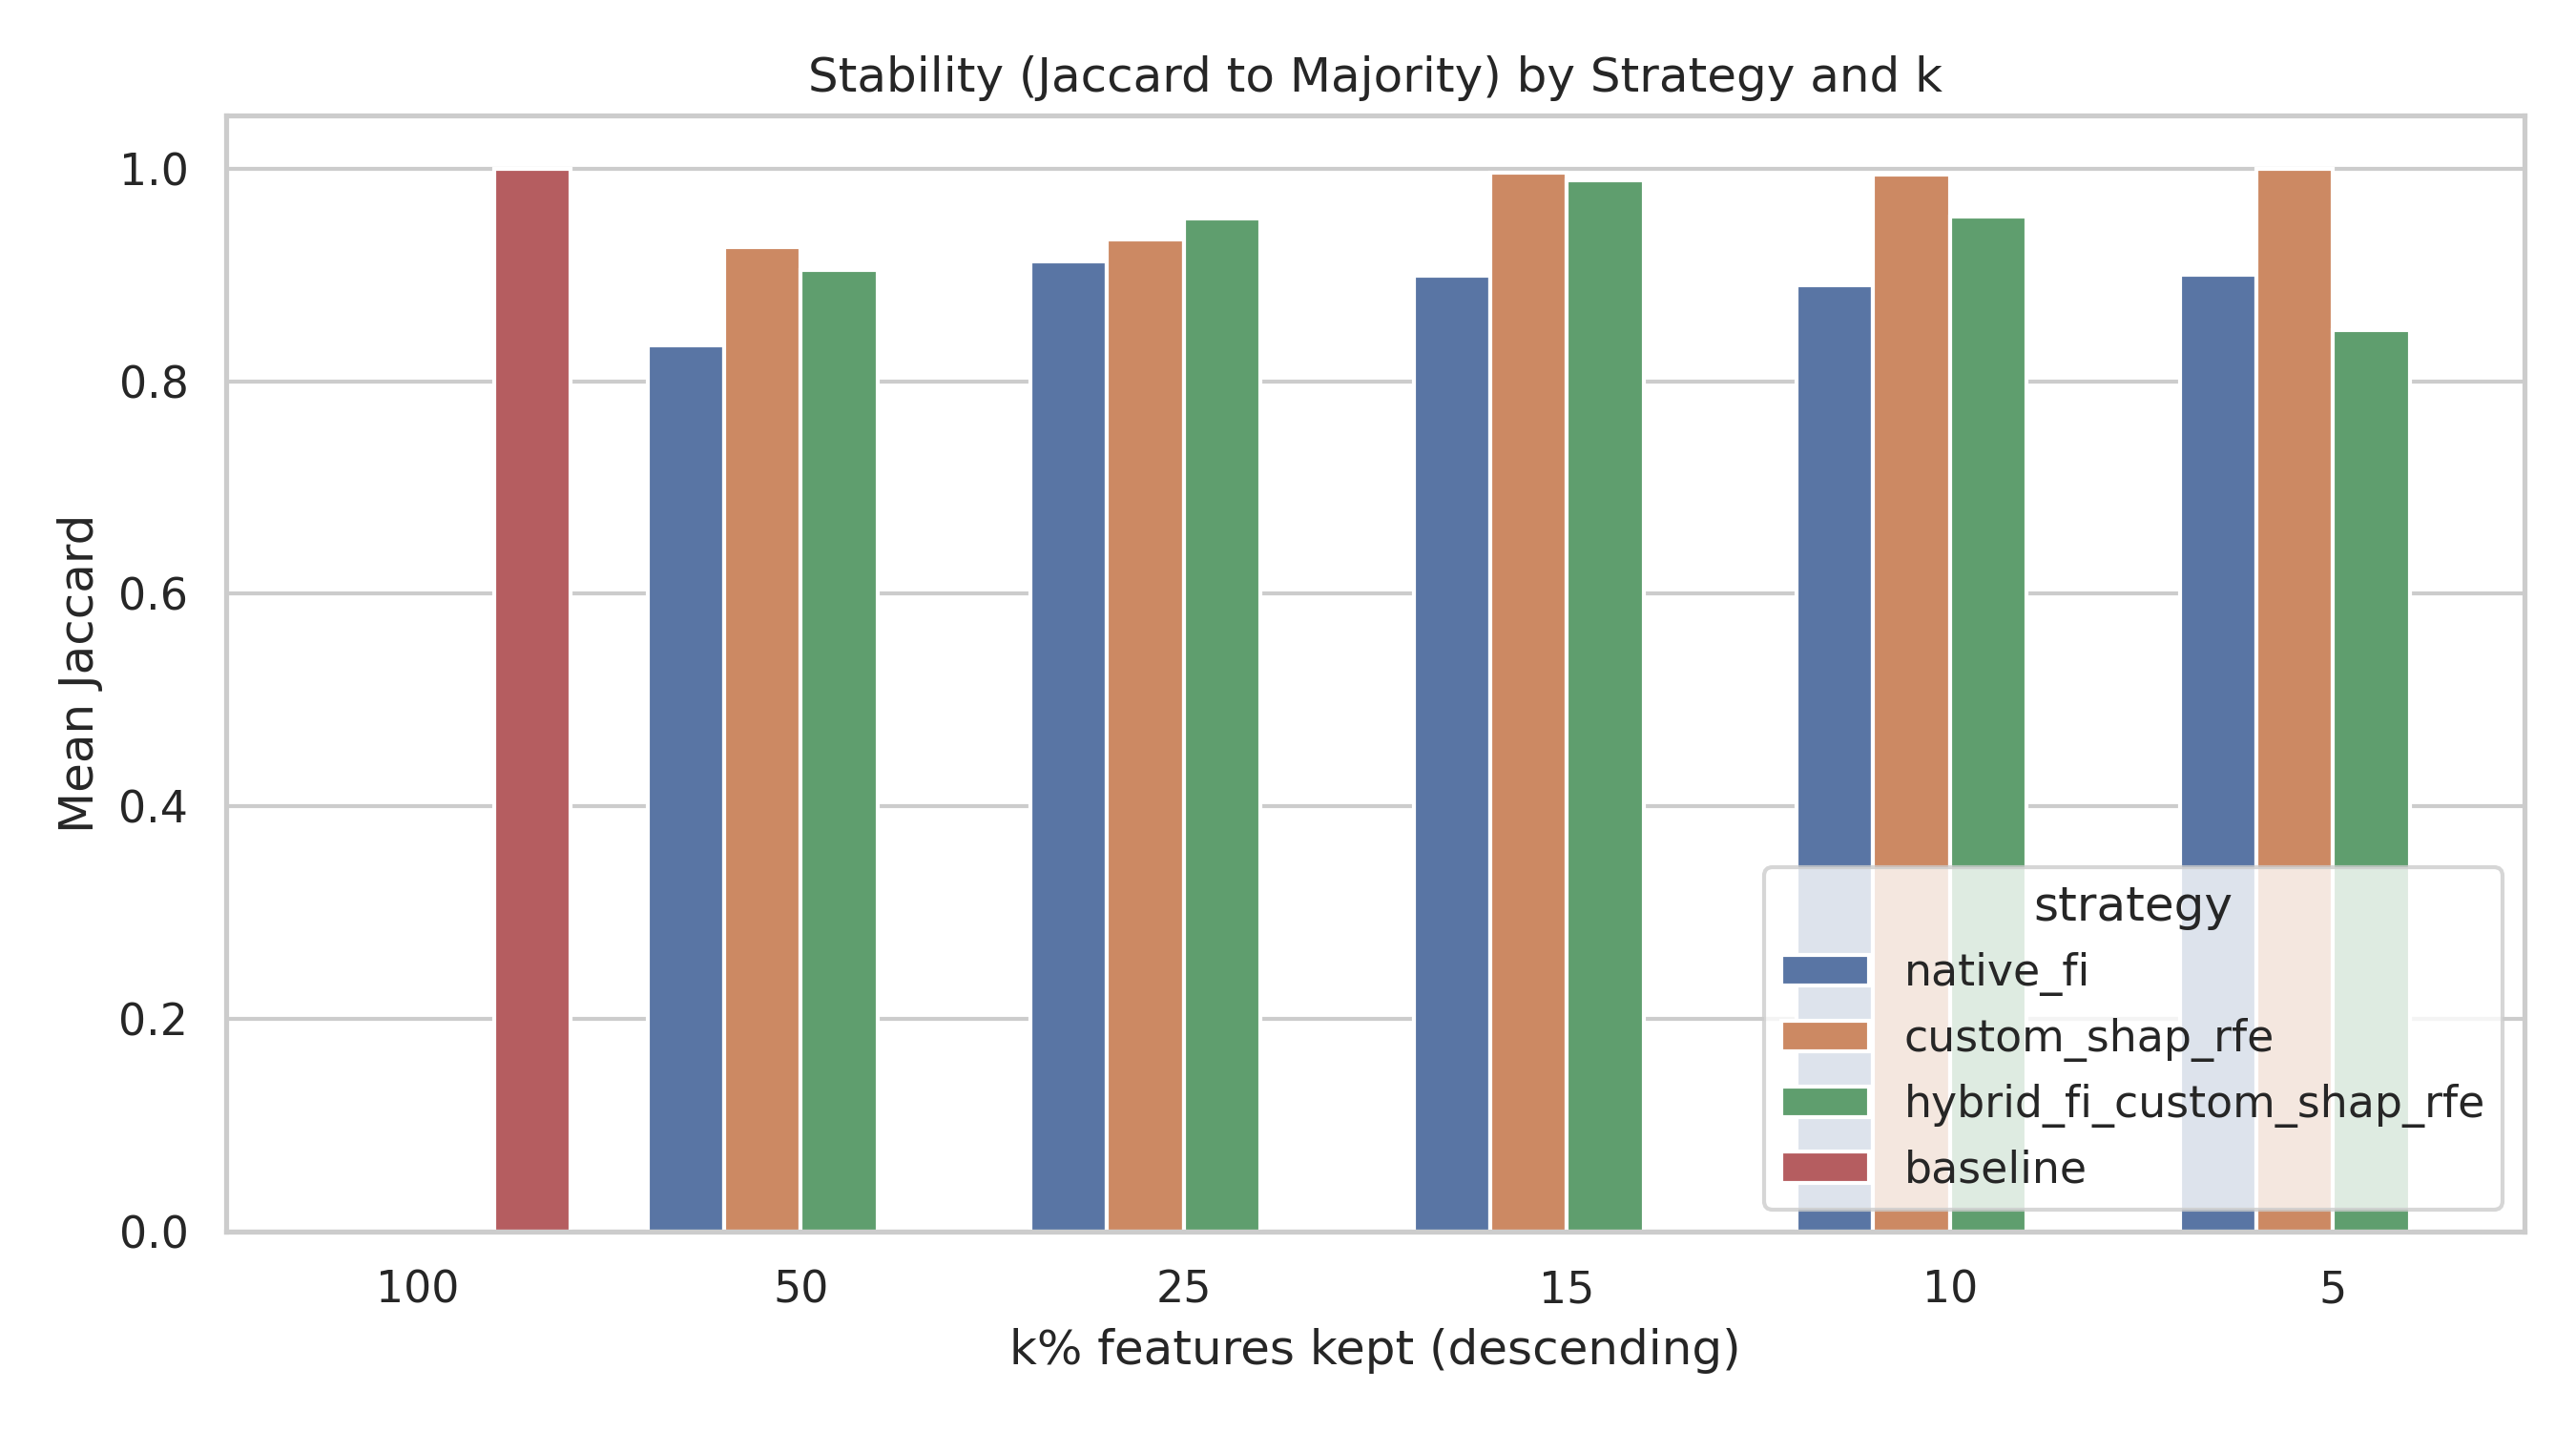
\includegraphics[width=0.48\textwidth]{../runs/exp3_run01/figures/exp3_stability_by_strategy_k.png}
    \caption{Selection stability in Stage~2: Superconductor (left) and Allstate (right).}
    \label{fig:stage2_stability}
\end{figure}

Stability follows expected patterns: lower at aggressive retention ($k=0.05$) and higher as more features are retained. Custom\_shap\_rfe shows notably high stability on Allstate at low $k$, suggesting that SHAP rankings are relatively consistent despite the model's stochasticity. The hybrid strategy's stability is comparable to simpler methods, providing no stability advantage to justify its cost.

\section{Synthesis and Hypothesis Evaluation}

The combined evidence from both stages supports the following conclusions:

\textbf{H1 (Competitive but non-dominant)}: \textit{Supported}. SHAP-based selection wins in 2 of 12 Stage~1 configurations, both with XGBoost. It is competitive but not dominant.

\textbf{H2 (Marginal gains at intermediate retention)}: \textit{Partially supported}. Small RMSE improvements appear at $k=0.25$ to $k=0.50$ in select cases (Allstate XGBoost with SHAP in Stage~1; custom\_shap\_rfe at $k=0.25$ in Stage~2 Allstate). However, these gains are minimal ($<1\%$ relative improvement).

\textbf{H3 (Substantial computational overhead)}: \textit{Supported}. The hybrid strategy consistently requires 20-30x more time than native\_fi with no systematic accuracy benefit. Even custom\_shap\_rfe, while faster, offers negligible advantage over native importance.

\textbf{H4 (Reduced stability at low retention)}: \textit{Partially supported}. Stability does decrease at low $k$ for all methods, but SHAP-based methods do not show dramatically worse stability than alternatives. In some cases (custom\_shap\_rfe on Allstate), SHAP stability is high.

\section{Threats to Validity}

Several limitations affect the generalizability of these findings:

\textbf{Dataset selection}: Four datasets cannot represent all tabular regression problems. Different domains or data characteristics might yield different conclusions.

\textbf{Hyperparameter choices}: Models were run with default or lightly-tuned hyperparameters. Joint optimization of feature selection and model hyperparameters might change relative rankings.

\textbf{Implementation details}: The custom SHAP-RFE and hybrid strategies are specific implementations. Alternative designs (e.g., different step sizes, pruning thresholds) might perform differently.

\textbf{Synthetic backfilling}: In Stage~1 data harmonization, some missing rows were interpolated. This caveat is acknowledged but does not affect the cleaner Stage~2 comparisons.

\section{Chapter Summary}

The experimental results demonstrate that SHAP-based feature selection, while theoretically principled and occasionally achieving the best RMSE, does not provide consistent practical advantages over simpler alternatives. Mutual Information and native tree importance frequently match or exceed SHAP performance at lower computational cost. The hybrid strategy, designed to combine the best of both worlds, instead combines computational expense with marginal performance. These findings suggest that practitioners should default to simpler methods and reserve SHAP-based selection for cases where its value has been demonstrated on the specific task at hand.
